\documentclass[review]{elsarticle}

\usepackage{lineno,hyperref}
\usepackage{algorithm}
\usepackage{algorithmic}
\usepackage{amsmath,amssymb}
\usepackage{graphicx}
\usepackage{subfig}
\usepackage{tabularx}
\usepackage[usenames,dvipsnames]{xcolor}
\usepackage{colortbl}
\usepackage{amsmath}
\usepackage{array}
\usepackage{booktabs}
\modulolinenumbers[5]

\journal{CIRP Journal of Manufacturing Science and Technology}

%%%%%%%%%%%%%%%%%%%%%%%
%% Elsevier bibliography styles
%%%%%%%%%%%%%%%%%%%%%%%
%% To change the style, put a % in front of the second line of the current style and
%% remove the % from the second line of the style you would like to use.
%%%%%%%%%%%%%%%%%%%%%%%

%% Numbered
%\bibliographystyle{model1-num-names}

%% Numbered without titles
%\bibliographystyle{model1a-num-names}

%% Harvard
%\bibliographystyle{model2-names.bst}\biboptions{authoryear}

%% Vancouver numbered
%\usepackage{numcompress}\bibliographystyle{model3-num-names}

%% Vancouver name/year
%\usepackage{numcompress}\bibliographystyle{model4-names}\biboptions{authoryear}

%% APA style
%\bibliographystyle{model5-names}\biboptions{authoryear}

%% AMA style
%\usepackage{numcompress}\bibliographystyle{model6-num-names}

%% `Elsevier LaTeX' style
\bibliographystyle{elsarticle-num}
%%%%%%%%%%%%%%%%%%%%%%%

\begin{document}

\begin{frontmatter}

\title{A Spatial AR System for Wide-area Axis-aligned Metric Augmentation of Planar Scenes} %\title{Elsevier \LaTeX\ template\tnoteref{mytitlenote}}
%\tnotetext[mytitlenote]{Fully documented templates are available in the elsarticle package on \href{http://www.ctan.org/tex-archive/macros/latex/contrib/elsarticle}{CTAN}.}

%% Group authors per affiliation:
\author{Michael Horn\'{a}\v{c}ek}\corref{mycorrespondingauthor}
\cortext[mycorrespondingauthor]{Corresponding author}
\ead{michael.hornacek@tuwien.ac.at}
\author{Hans K\"{u}ffner-McCauley}
\author{Majesa Trimmel}
\author{Patrick~Rupprecht}
\author{Sebastian Schlund}
\address{Human Centered Cyber Physical Production and Assembly Systems, Institute for Management Sciences, TU Wien, Vienna, Austria}

\begin{abstract}
Augmented reality (AR) promises to enable use cases in industrial settings that include the embedding of assembly instructions directly into the scene, potentially reducing or altogether obviating the need for workers to refer to such instructions in paper form or on a statically situated screen. \textit{Spatial} AR, in turn, is a form of AR whereby the augmentation of the scene is carried out using a projector, with the advantage of rendering the augmentation visible to all onlookers simultaneously without calling for any to hold a handheld device such as a tablet or for each to wear some form of head-mounted display. In carrying out spatial AR, however, care must be taken to appropriately warp the image to be projected such that it, when projected, appear free of projective distortions to the viewer. For planar scene geometry (such as a floor, wall, or table), a manual process called keystone correction can be used to carry out an appropriate corrective image warp, a process that can be cumbersome. Another drawback of conventional spatial AR relying only on a single projector is that it is capable of augmenting only the portion of the scene within the projector's static field of view, thereby hindering its applicability to use cases calling for augmentation of wide areas such as a factory floorspace.

We propose a spatial AR system for wide-area metric augmentation of planar scene surfaces that produces the effect of keystone correction analytically as a function of the relative geometry of the projector and scene plane, using a projector equipped with a steerable mirror to direct the projection across varying target locations and a camera facing the scene plane in support of calibrating the system. Our system renders the placement of augmentations in the scene more intuitive than manual keystone correction in two ways. First, (i) the horizontal and vertical axes of the desired augmentations is carried out in accordance with the horizontal and vertical image axes of the camera, thereby making setting those axes as simple as appropriately rotating the camera relative to the scene plane, and thereby providing a consistent axial reference frame across all target locations. Second, (ii) the desired dimensions of the projected augmentations are specified in metric terms, thereby providing for consistent scaling, likewise across all target locations. %Our system produces such augmentations accurately, with compelling time savings relative manual keystone correction.
\end{abstract}

\begin{keyword}
Spatial augmented reality (SAR) \sep computer vision \sep steerable mirror projector \sep projector-camera calibration \sep Industry 4.0
\end{keyword}

\end{frontmatter}

\linenumbers

\section{Introduction}\label{sec:intro}

Augmented reality (AR) \cite{van2010survey,zhou2008trends} promises to enable use cases in industrial settings that include the embedding of assembly instructions directly into the scene~\cite{schlund2018moglichkeiten,uva2018evaluating,masood2019augmented,gattullo2019towards,aschenbrenner2019comparing,mayrhofer2019one,rupprecht2020information,Rupprecht2021}, potentially reducing or altogether doing away with the need for workers to refer to such instructions in paper form or on a statically situated screen. Typically, AR works by embedding the augmentation in imagery of the scene acquired from the viewpoint of a single individual, with the resulting augmented image in turn displayed typically using some form of handheld or head-mounted display. Handheld devices such as tablets do not enable the user to work hands-free while using the device, or force the user to wear additional gear. Reliance on head-mounted displays has two adverse consequences of its own: a head-mounted display must be worn by each individual wishing to partake in the augmentation, and such a head-mounted display---in some cases taking the form of a helmet in order to house multiple sensors in support of accurately tracking the viewpoint of the viewer relative to the scene---can be obtrusive. A HoloLens 2 (Microsoft Corporation, USA), for instance, is such a head-mounted display; at a weight of 566~grams \cite{hololens}, it places an additional ergonomic load on the worker, in particular if worn over a longer duration or in bent positions.

\begin{figure}[t]
    \centering
    \subfloat[\centering Original image.]{\raisebox{10mm}{
\includegraphics[width=5cm]{images/projim.png}}}
    \qquad
    \subfloat[\centering Projection of original image to target location in scene plane (view directly downwards to scene plane).]{{
\includegraphics[width=6cm]{images/proj_projim_full_.png}}}
    \caption{Na\"ive projection to a given target location in the scene plane (e.g., the floor, a wall, or table) if not facing the scene plane directly. (a) Original image, which we wish to project to the scene plane. (b) Projecting the original image to the scene plane from the viewpoint of the projector (shown as a frustum in the bottom left, in black with up vector red) directed to the target location introduces projective distortions if the projector does not face the scene plane directly (as is the case here), with orientation and scale of the augmentation varying in the scene plane as a function of target location.}
    \label{fig:proj}
\end{figure}

In turn, a form of augmented reality referred to as \textit{spatial} AR\cite{bimber2019spatial} is carried out not by embedding the augmentation in an image of the scene as with a head-mounted or handheld display, but by projection to the scene itself, thus eliminating the aforementioned problems. Spatial AR thus turns surfaces such as the object being manufactured, a desk, the floor, a wall, or even the ceiling (considering overhead work) into displays. Information provision---of the work plan or of quality-related information---can be carried out by projection to the given workspace, while directly referring to exact positions within that workspace. Moreover, the fact that this information can be viewed by multiple users simultaneously serves to facilitate collaboration \cite{aschenbrenner2019comparing}.

\begin{figure}[t]
    \centering
    \subfloat[\centering Our warped image.]{\raisebox{10mm}{
\includegraphics[width=5cm]{images/projim_warped_scaled.png}}}
    \qquad
    \subfloat[\centering Projection of our warped image to target location in scene plane (view directly downwards to scene plane).]{{
\includegraphics[width=6cm]{images/proj_projim_waped_full_.png}}}
    \caption{Projection to a given target location in the scene plane, correcting for projective distortions in terms of a \textit{virtual} projector placed and utilized using our approach. (a) Original image (cf.\ Figure~\ref{fig:proj}(a)) warped using our approach. (b) Projecting the warped image to the scene plane from the viewpoint of the projector (bottom left, frustum in black with up vector red; same as in Figure~\ref{fig:proj}(b)) directed to the target location has the effect of projecting the \textit{original} image from the viewpoint of a virtual projector (center, frustum in gray with up vector red). This renders the projection free of projective distortions, aligned with the axes of the virtual camera, and at the desired metric scale. Note that black pixels will in effect be ignored by the projector.}
    \label{fig:warp}
\end{figure}

While interest in spatial AR in industrial settings has been growing, its deployment in industrial settings remains well behind that of wearable AR systems such as handhelds or head-mounted displays. One of the main shortcomings of typical projector-based spatial AR relative to AR relying on wearables is the ability to project augmentations only within the projector's own static field of view. Here, dynamic projection systems---using steerable mirror heads to direct the projection across wider areas---has the potential to bridge the gap to wider industrial penetration. Yet the increase in the area to be covered comes with noteworthy challenges in terms of preparing the augmentations, in particular as the number of target locations in the scene becomes larger than a small handful. Considering a planar surface to be augmented (e.g., a floor, wall, or table), unless the projector faces the surface frontally, the bounds of a projected rectangular image will not appear rectangular, but will instead be subject to projective distortions (cf.\ Figure~\ref{fig:proj}). Such distortions can be corrected for by carrying out a cumbersome manual process referred to as keystone correction---involving warping an image by perturbing its corners until the desired effect is produced when projected to the scene---to appropriately warp the image to be projected, often using software bundled with the projector. Automating this manual, time-consuming, and error-prone process significantly reduces the time needed for the industrial engineering of a spatial AR application and therefore has potential to promote adoption by industry. Especially manufacturing processes of large products that remain at a static mounting position during the assembly process---i.e., industrial site assembly---offer a significant application potential for the use of spatial AR as part of worker assistance systems \cite{mayrhofer2019one}.

Our contribution is to propose a wide-area spatial AR system for planar scenes that produces the effect of keystone correction analytically, free of any manual interaction. Notably, we do this in a manner placing the $X$- and $Y$-axes of the augmentation in accordance with the $X$- and $Y$-axes of a camera placed to face downwards towards the scene plane (cf.\ Figure~\ref{fig:eval}(a)). In what follows,  \textit{we shall refer to this camera as `downwards facing'} for brevity, in quotes since the pose of the camera is likely to deviate at least gently from facing downwards to the scene plane directly (an effect for which we shall carry out a correction). Relying on the placement of the `downwards-facing' camera thus facilitates placement of augmentations, since setting the $X$- and $Y$-axes of augmentations with respect to the scene plane thus reduces to appropriately rotating the `downwards-facing' camera relative to the scene plane. We compute our corrective image warp for a given target location by warping the image to be projected using a plane-induced homography computed to produce the effect of projecting the image not from the actual projector viewpoint, but in accordance with the viewpoint of a \textit{virtual} projector (cf.\ Figure~\ref{fig:warp}). We place this virtual projector to (i) face directly downwards to the target location in the scene plane and (ii) rotate its axes to match those of the virtual camera. Moreover, our system enables specifying the dimensions of augmentations in metric terms, which we achieve by placing the virtual projector at the appropriate height above the scene plane. Finally, our system is set up for use with a projector equipped with a steerable mirror in a manner that does not call for explicitly modeling the action of the steerable mirror on the projector, thereby enabling wide-area applications exceeding the immediate field of view of the projector without needing to rely on multiple projectors.

%This makes setting those axes particularly easy from the user viewpoint, since it reduces to appropriately rotating the `downwards-facing' camera relative to the scene plane. Because we wish to set the principal axes of our augmentations in terms of a rotation about the normal vector of the scene plane,  To compensate for the likely possibility that the camera not face downwards to the scene plane precisely, we rotate the recovered `downwards-facing' camera to face downwards directly, yielding what we refer to as the \textit{virtual} camera.

\subsection{Related Work}

An early spatial AR system explicitly using a projector mounted with a steerable mirror is the IBM Everywhere Displays prototype of Pinharez \cite{pinhanez2001everywhere}. For the purposes of the prototype, a projector mounted with a steerable mirror was set up with a camera to demonstrate a variety of use cases, including collaborative assembly encompassing the projection of assembly instructions and an interactive projected user interface \cite{kjeldsen2002interacting,pinhanez2003applications}. The authors, however, carry out keystone correction manually, by interactively adjusting for the position and orientation of a virtual scene plane and a scaling factor and computing a corresponding 2D homography accordingly. %Rather than rely on a steerable mirror to support spatial AR to multiple locations using a single projector, some works mount the projector and a camera on a rigid rig and subject the rig to motion \cite{ehnes2004projected,borkowski2004spatial,butz2006applying}. Steering only a mirror, however, places humbler requirements on the system from a hardware standpoint than if an entire camera-projector rig is to be subject to rigid motion.

More generally, keystone correction for planar scenes can be said to reduce to computing a 2D homography \cite{Hartley2004}, an invertible transformation that preserves colinearity and is thus fittingly alternatively referred to as a `colineation'; this is the case whether computing the homography relies on manual interaction as in the case of Pinharez, or is obtained free of manual interaction as in ours. The intuition for why it is that a transformation that preserves colinearity---i.e., maps lines to lines---can serve to model an appropriate corrective image warp can be drawn from considering a planar chessboard pattern: looking at a chessboard from an oblique angle, one observes that lines parallel in the chessboard appear to meet in respective vanishing points, yet remain lines; looking at the same chessboard frontally with respect to the plane of the chessboard, lines parallel in the chessboard appear parallel in the image (i.e., they are said to meet `at infinity'). To warp an image of the chessboard acquired at one angle such that the lines of the chessboard appear as if the chessboard were acquired at another angle accordingly calls for a transformation that maps lines to lines; it therefore follows that there exists a homography that models that transformation.

One way to compute a homography is by identifying at least four correspondences between pixel positions in two images of a planar surface \cite{Hartley2004}. The keystone correction approach of Sukthankar \textit{et al.} \cite{sukthankar2001smarter} reduces to using a segmentation approach to identify the four corners of projection screen in an image acquired by a camera, and computing a homography that maps the resulting four corners of the projection screen to the four corners of the projector's image plane. Additional sensors can be used to inform the computation of a homography; Raskar and Beardsley \cite{raskar2001self} use a tilt sensor to recover the projector's gravity (i.e., down) vector, which they use to carry out a rotational correction in projecting to a wall. Still another way to compute a homography is as a function of a plane and a pair of pinhole cameras; the effect produced by the homography is one of projecting an image to the plane from the viewpoint of the one camera, and acquiring the projected image from the viewpoint of the other. Such a homography is said to be `induced' by a plane \cite{Hartley2004}. We exploit the fact that cameras and projectors alike can be modeled using a pinhole camera model \cite{bimber2019spatial}, proceed to recover the relative geometry relating the scene plane and projector, and compute a particular form of plane-induced homography to effect the intended corrective image warp, yet additionally taking into account both desired in-plane orientation and metric scale.

\section{Approach}

Correcting for projective distortions of the sort outlined in Section~\ref{sec:intro}---and exemplified in Figure~\ref{fig:proj}---can be achieved by means of an appropriate plane-induced homography \cite{Hartley2004}, computed by modeling the manner in which the respective rays through the pixels of the projector's image plane fan out into the scene (i.e., by `calibrating' the projector) and the geometry of the scene itself (i.e., by recovering the scene plane relative to the projector) within at least the projector's field of view. This is because the scene point `illuminated' by a pixel in the projector's image plane can be recovered by intersecting its corresponding ray with the geometry of the scene plane; modeling the geometry that relates projector and scene plane thus enables one to reason about the problem of correcting for distortions in terms of geometry. To model this interaction, we (i) carry out a one-time projector calibration, which in our approach calls for additionally calibrating a camera facing downwards to the scene plane and includes recovery of the scene plane. Next, we use the relative camera-projector-scene plane geometry to (ii) compute a plane-induced homography that warps the image to be projected in a manner that it appear undistorted to the viewer, placed in alignment with the axes of a proxy image of the scene, and at the desired metric scale. These two points are treated in Sections~\ref{sec:approach:geometry} and \ref{sec:approach:homography}, respectively.

\subsection{Recovering Geometry}\label{sec:approach:geometry}

\begin{figure}[t]
    \centering
    \subfloat[\centering Projector calibration image (2D pattern position detections overlain).]{{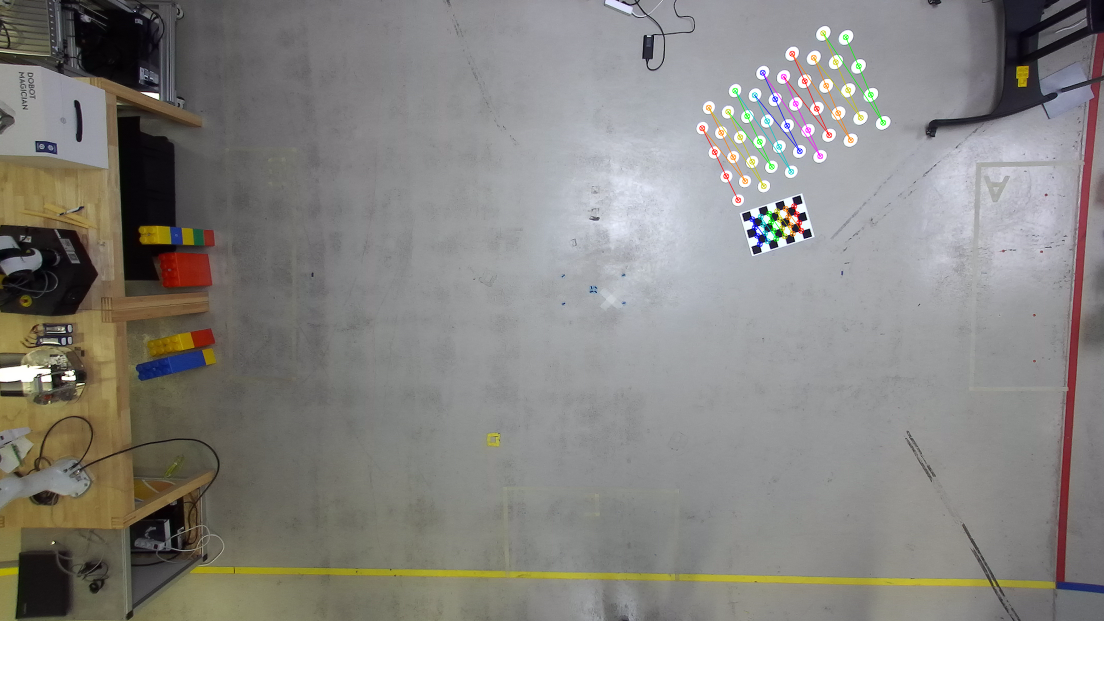
\includegraphics[width=5.15cm]{images/detections_.png}}}
    \quad
    \subfloat[\centering Recovered 3D positions corresponding to projector calibration image for use in projector calibration (red, in scene plane).]{{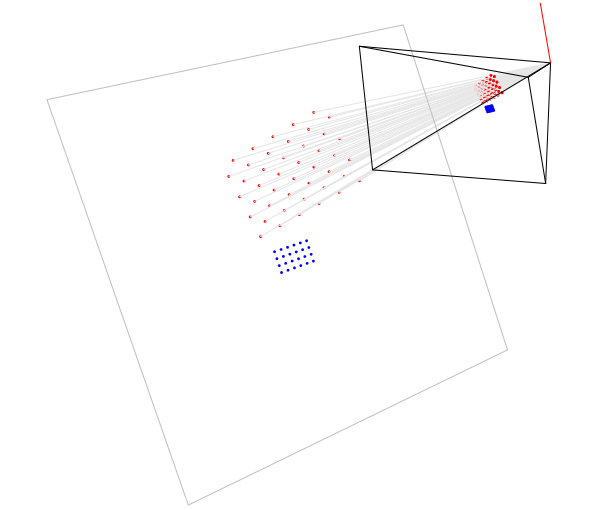
\includegraphics[height=3.7cm]{images/2d3d.png}}}
    \caption{Obtaining the 3D positions of the 2D-3D correspondences for use in projector calibration. (a) For each target location, a projector calibration image is acquired from the viewpoint of the `downwards-facing' camera, containing a projected asymmetric circle pattern at the target location and a chessboard pattern placed on the floor nearby. Circle pattern center points and chessboard corners detected automatically (overlain for illustration). (b) Given a projector calibration image, the scene plane is recovered in the coordinate frame of the camera (black with up vector red) via spatial resection with respect to 2D-3D correspondences obtained using the chessboard pattern (blue); the 3D positions of the 2D-3D correspondences to be used in calibrating the projector (red, in scene plane) are obtained by intersection with the scene plane of the back-projections (rays, likewise gray) of the 2D center points of the circle pattern detected in the image plane of the camera.} %The corresponding 2D positions are detected in the image of the asymmetric circles pattern image projected by the projector (not shown). The `downwards-facing' camera is shown relative to the scene plane in terms of its camera frustum (black, with up vector in red).
    \label{fig:2d}
\end{figure}

Calibration of a projector (or camera) in the sense we employ the term here\footnote{We are referring to a geometric calibration; not, e.g., to a color calibration.} renders one able to project a scene point~$\mathbf{X} \in \mathbb{R}^3$ to its corresponding pixel~$\mathbf{x} \in \mathbb{R}^2$ in the projector's (or camera's) image plane, or to compute the `back-projection' of $\mathbf{x}$, i.e., the ray from the projector's (or camera's) center of projection through $\mathbf{x}$ along which a projecting point~$\mathbf{X}$ must lie. Such a calibration can be expressed in terms of (i) a $3~\times{}~3$ calibration matrix~$\mathtt{K}$ derived from the projector's (or camera's) focal length~$f$ and principal point~$\mathbf{p}_0 = (x_0, y_0)^\top \in \mathbb{R}^2$ \cite{Hartley2004}, and (ii)~the coefficients of a lens distortion model used to correct for radial or tangential distortions caused by the lens system \cite{duane1971close,weng1992camera}; the calibration matrix~$\mathtt{K}$ is then
\begin{equation}
\mathtt{K} = \begin{bmatrix}
f & 0 & x_0 \\
0 & f & y_0 \\
0 & 0 & 1
\end{bmatrix},
\end{equation}
where $f$, $x_0$, and $y_0$ are each expressed in units of pixels. The calibration matrix~$\mathtt{K}$ models a so-called pinhole camera \cite{Hartley2004}; such a model is applicable to an image acquired using a real-world camera assuming the image has in a prior step been corrected for lens distortion effects. %, by having applied the appropriate lens distortion model coefficients.

A camera can be calibrated by (i) establishing 2D-3D correspondences between pixels in the camera's image plane and the corresponding points in the scene, and on (ii) using those correspondences as input to an optimization procedure that relies on bundle adjustment \cite{triggs1999bundle} to output maximum likelihood estimates of the calibration matrix, the associated lens distortion model coefficients, and, for each calibration image, the pose (i.e., position and orientation) of the camera relative to the 3D scene points from among the 2D-3D correspondences \cite{Hartley2004,zhang2000flexible}. Calibration images containing a calibration surface such as a chessboard pattern of known dimensions and scale are acquired from varying viewpoints using the camera, to be used to establish the 2D-3D correspondences~$\{\mathbf{x}_{i,j} \leftrightarrow \mathbf{X}_{i,j}\}$, $i \in \{ 1, \dots, n_\text{pt} \}, j \in \{ 1, \dots, n_\text{im} \}$, where $n_\text{pt}$ gives the number of correspondences obtained from one calibration image of the pattern, $n_\text{im}$ the number of such images, and $\mathbf{X}_{i,j} = \mathbf{X}_{i,j'}$, for $j, j' \in \{ 1, \dots, n_\text{im} \}$. Bundle adjustment is then used to obtain the maximum likelihood estimates~$(\hat{\omega}, \hat{\mathtt{K}}, \{(\hat{\mathtt{R}}_j, \hat{\mathbf{t}}_j)\}), j \in \{ 1, \dots, n_\text{im} \}$ of the lens distortion model coefficients~$\omega$, calibration matrix~$\mathtt{K}$, and rigid body transformations~$(\mathtt{R}_j, \mathbf{t}_j), j \in \{ 1, \dots, n_\text{im} \}$. These are obtained using bundle adjustment by minimizing the cumulative reprojection error
\begin{equation}
\sum_{i=1}^{n_\text{pt}} \sum_{j=1}^{n_\text{im}} d_{\hat{\omega}}(\mathbf{x}_{i,j}, \hat{\mathbf{x}}_{i,j}'),
\label{re}
\end{equation}
where $\hat{\mathbf{x}}_{i,j}' \in \mathbb{R}^2$ gives the projection of the point~$\mathbf{X}_{i,j} \in \mathbb{R}^3$ to the image plane of the camera underlying the $j^{\text{th}}$~calibration image, subject to the maximum likelihood estimates $\hat{\mathtt{K}}, (\hat{\mathtt{R}}_j, \hat{\mathbf{t}}_j)$. The function~$d_{\hat{\omega}}$, in turn, is a function that first (i) corrects $\mathbf{x}_{i,j}, \hat{\mathbf{x}}_{i,j}'$ for lens distortions in accordance with the maximum likelihood estimate of the lens distortion model coefficients~$\hat{\omega}$ \cite{duane1971close,weng1992camera}, and then (ii) computes a distance in pixels with respect to two resulting corrected positions. More generally, the projection~$\mathbf{x}' \in \mathbb{R}^2$ of a point~$\mathbf{X} \in \mathbb{R}^3$ to the image plane of a camera given calibration matrix~$\mathtt{K}$ and pose~$(\mathtt{R}, \mathbf{t})$ is given by
\begin{equation}
(\mathbf{x}'^\top, 1)^\top \sim \mathtt{K}(\mathtt{R}\mathbf{X} + \mathbf{t}) \in \mathbb{P}^2,
\end{equation}
where $\mathtt{R}\mathbf{X} + \mathbf{t} \in \mathbb{R}^3$ expresses $\mathbf{X}$ in the coordinate frame of the camera. Inverting the rigid body transformation~$(\mathtt{R}_j, \mathbf{t}_j)$ gives the pose~$(\mathtt{R}_j^{-1}, -\mathtt{R}_j^{-1}\mathbf{t}_j^{})$ of the $j^{\text{th}}$~camera relative to the 3D scene points of the calibration pattern, with $-\mathtt{R}_j^{-1}\mathbf{t}_j^{} \in \mathbb{R}^3$ the corresponding center of projection.

Calibrating a projector \cite{moreno2012simple,zhang2009projector,zhang2006novel} can be carried out in precisely the same manner as calibrating a camera insofar as step (ii) is concerned; the major difference in projector calibration relative to the calibrating a camera then concerns the manner in which 2D-3D correspondences are identified, i.e., between pixels in the image plane of the \textit{projector} and the corresponding points in the scene. What remains of this section is concerned primarily with the recovery of 2D-3D correspondences, first in support of calibrating the `downwards-facing' camera (giving the camera calibration matrix~$\mathtt{K}_\text{cam}$), then---in a manner that makes use of $\mathtt{K}_\text{cam}$---for calibrating the projector (giving the projector calibration matrix~$\mathtt{K}_\text{proj}$ and the projector poses~($\hat{\mathtt{R}}_j, \hat{\mathbf{t}}_j)$, for each projector calibration image).

\paragraph{2D-3D correspondences for camera calibration} We recover 2D-3D correspondences in support of calibrating the `downwards-facing' camera by relying on a planar calibration surface to automatically identify correspondences between the 3D points on the calibration surface and their 2D correspondences in the image plane. The classical calibration surface is a chessboard pattern, and is such a pattern that we use as well. The 3D corner points of the chessboard are obtained \textit{a priori} in a coordinate system defined in the plane of the chessboard\footnote{E.g., $(0,0,0), (1.5,0,0), (3,0,0), \dots, (9,7.5,0)$ for a chessboard with $7~\times{}~6$ corners ($8~\times{}~7$ squares), with each square of length and width of 1.5 unit, respectively. Note that the units of the chessboard's 3D points give the units of the camera calibration, and---since our projector calibration relies on the camera calibration---the units of the projector calibration as well.}, requiring knowledge only of the dimensions of the chessboard pattern and of the length of a side of a chessboard square. The corresponding 2D points are obtained, in the same order, using a specialized algorithm \cite{bradski2000opencv}. A set of calibration images is acquired, each with the calibration pattern visible in a different part of the image plane, and such that the center and all corners and edges of the image plane are covered, the camera's autofocus setting be off, and the camera's zoom factor remain fixed. 2D-3D correspondences are then recovered for each calibration image, respectively, and the resulting list of correspondences is used to recover the camera calibration matrix~$\mathtt{K}_\text{cam}$. 

\paragraph{2D-3D correspondences for projector calibration} For projector calibration, we obtain the 2D-3D correspondences by \textit{projecting} a calibration pattern to the scene plane, once for each target location. Since we know that the 3D positions of the projected pattern must lie in the scene plane, we can recover the 3D correspondence of a pattern point detected in the 2D image plane of the `downwards-facing' camera by intersecting the back-projection of the 2D position with the scene plane. We reuse the chessboard pattern---used above for camera calibration---to recover the scene plane locally to each target location via spatial resection \cite{Hartley2004}, by placing the chessboard pattern on the floor near the projected pattern and using the resulting 2D-3D chessboard correspondences as input to a PnP algorithm \cite{collins2014infinitesimal}. While a single image of such a chessboard pattern placed on the floor could be sufficient if the floor is even, we recover a scene plane per projector calibration image to account for the possibility of an uneven floor. Since our projector calibration images thus already contain a chessboard, we choose an alternative calibration pattern as the pattern to project, namely an asymmetric circle pattern. We again use a specialized algorithm \cite{bradski2000opencv} to obtain the circle centers of the asymmetric circle pattern, capable of recovering circle centers even under projective distortions. 

Given a projector calibration image acquired using the `downwards-facing' camera, we detect the circle centers of the \textit{projected} asymmetrical circle pattern (cf.\ Figure~\ref{fig:2d}(a)); given the scene plane and such a 2D circle center $\mathbf{x}$, we obtain its 3D correspondence by intersecting the back-projection
\begin{equation}
\mathtt{K}_\text{cam}^{-1}(\mathbf{x}^\top, 1)^\top \in \mathbb{P}^2
\end{equation}
of $\mathbf{x}$ with the recovered scene plane (cf.\ Figure~\ref{fig:2d}(b)). We obtain the 2D positions of the 2D-3D correspondences by simply running the algorithm for detecting circle centers on the original asymmetric circles pattern image (i.e., the one we feed to the projector). Since---as in the case of recovering chessboard pattern corners---the algorithm that yields 2D circle centers does so in a consistent ordering, we thus obtain respective 2D-3D correspondences for each projector calibration image, which we use to recover the projector calibration matrix~$\mathtt{K}_\text{proj}$.

Recall that the pose~($\hat{\mathtt{R}}_j, \hat{\mathbf{t}}_j)$ of the projector, for each projector calibration image~$j$, is provided alongside $\mathtt{K}_\text{proj}$, relative to the 3D points of the pattern and thus in the coordinate frame of the `downwards-facing' camera. Note that for a fixed projector with steerable mirror, given a projector calibration image, the recovered projector's pose is the pose the projector would have to have had to project to the given target location \textit{in the absence of the mirror} (i.e., facing directly towards the target location). It is in this sense that our system is able to handle a projector equipped with a steerable mirror, without need for modeling the steerable mirror explicitly.

\subsection{Correcting for Projective Distortion}\label{sec:approach:homography}

\begin{figure}[t]
    \centering
    \subfloat[\centering Oblique view (annotated).]{{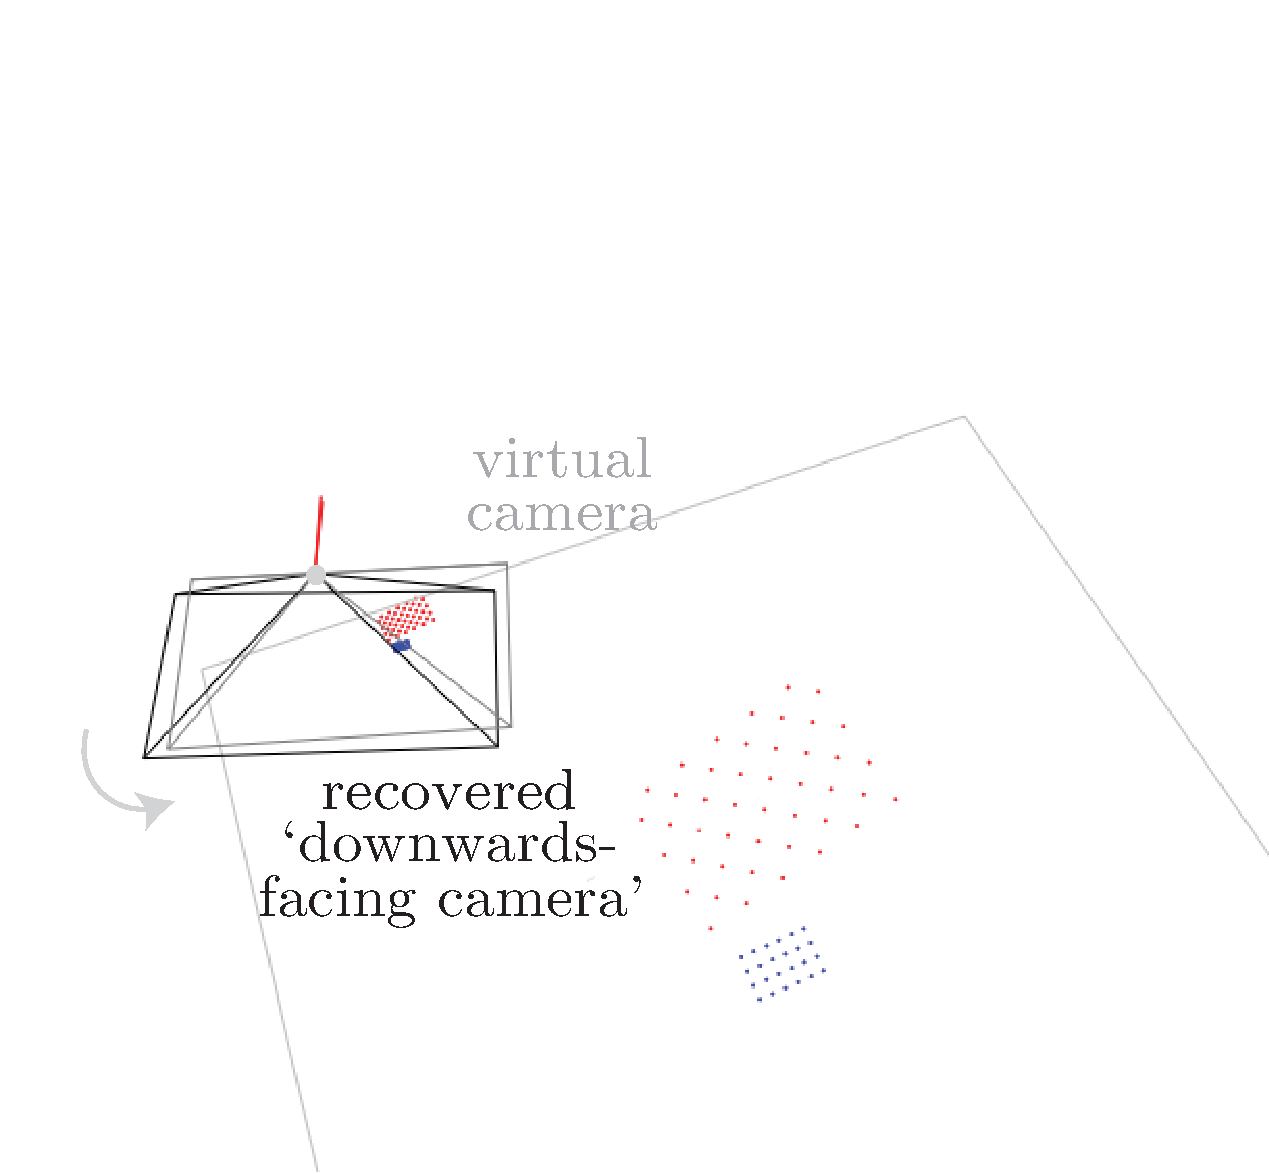
\includegraphics[height=5.25cm]{images/3_cam_.pdf}}}
    \qquad
    \subfloat[\centering View directly downwards to scene~plane.]{{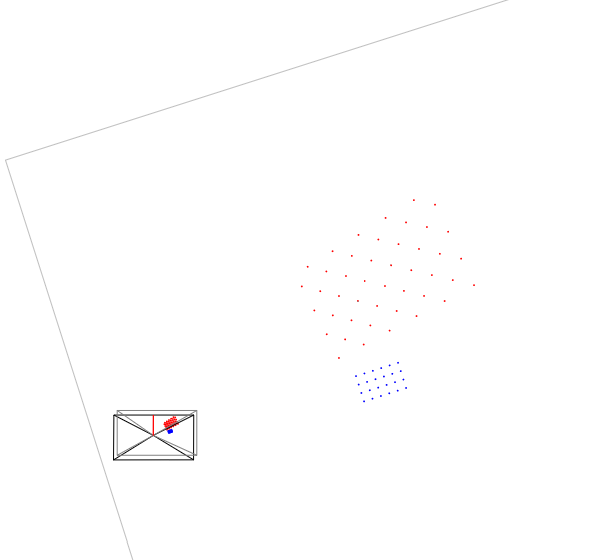
\includegraphics[height=5.25cm]{images/3_above3_cam.png}}}
    \caption{Obtaining the virtual camera. Our physical `downwards-facing' camera---placed to face downwards towards the scene plane, and in terms of whose rotation relative to the normal vector of the scene plane we wish to orient our augmentations---is almost certain to not face downwards towards the scene plane precisely. Accordingly, we rotate the recovered `downwards-facing' camera (frustum in black) about its center of projection such that its optical axis be made parallel with the scene plane's normal, with respect to the minimum arc-length rotation relating the two.} %It is then, for each respective target location, the $X$- and $Y$-axes of the resulting \textit{virtual} camera (gray) that we subsequently use to orient the virtual projector (cf.\ Figure~\ref{fig:virtualproj}) in terms of which the augmentation is to appear to be projected, which is itself placed to face downwards towards the scene plane precisely. The virtual projector is thus rendered fronto-parallel with the ground plane and axially aligned with the virtual camera. This rotated camera is our virtual camera, and it is the orientation of the virtual camera that we subsequently use to orient our virtual projector.
    \label{fig:virtualcam}
\end{figure} 

If the projector is calibrated and its pose relative to the scene plane is known, a `virtual' projector (with the same calibration $\mathtt{K}$ and lens distortion model coefficients) can be placed elsewhere relative to the scene plane. If we for a moment imagine that the projector---at its recovered pose---functions as a camera,\footnote{Recall that the calibration matrix~$\mathtt{K}$ enables computing (i) the projection of a scene point to the image plane (the function of a camera), or (ii) the back-projection of a pixel in the image plane, giving a ray into the scene (along which a projector illuminates the scene with the given pixel).} then (i) projecting an image to the scene plane \textit{from the viewpoint of the virtual projector} and (ii) acquiring the resulting projected image \textit{from the viewpoint of the recovered projector} gives the desired corrective warp (cf.\ Figure~\ref{fig:warp}). Projecting an image warped in this manner to the scene plane from the viewpoint of the recovered projector then has the same effect as projecting the original image to the scene plane from the viewpoint of the virtual projector. This warp can be effected using a plane-induced homography, computed analytically as a function of the scene plane, the projector, and the virtual projector.

\begin{figure}[t]
    \centering
    \subfloat[\centering Oblique view (annotated).]{{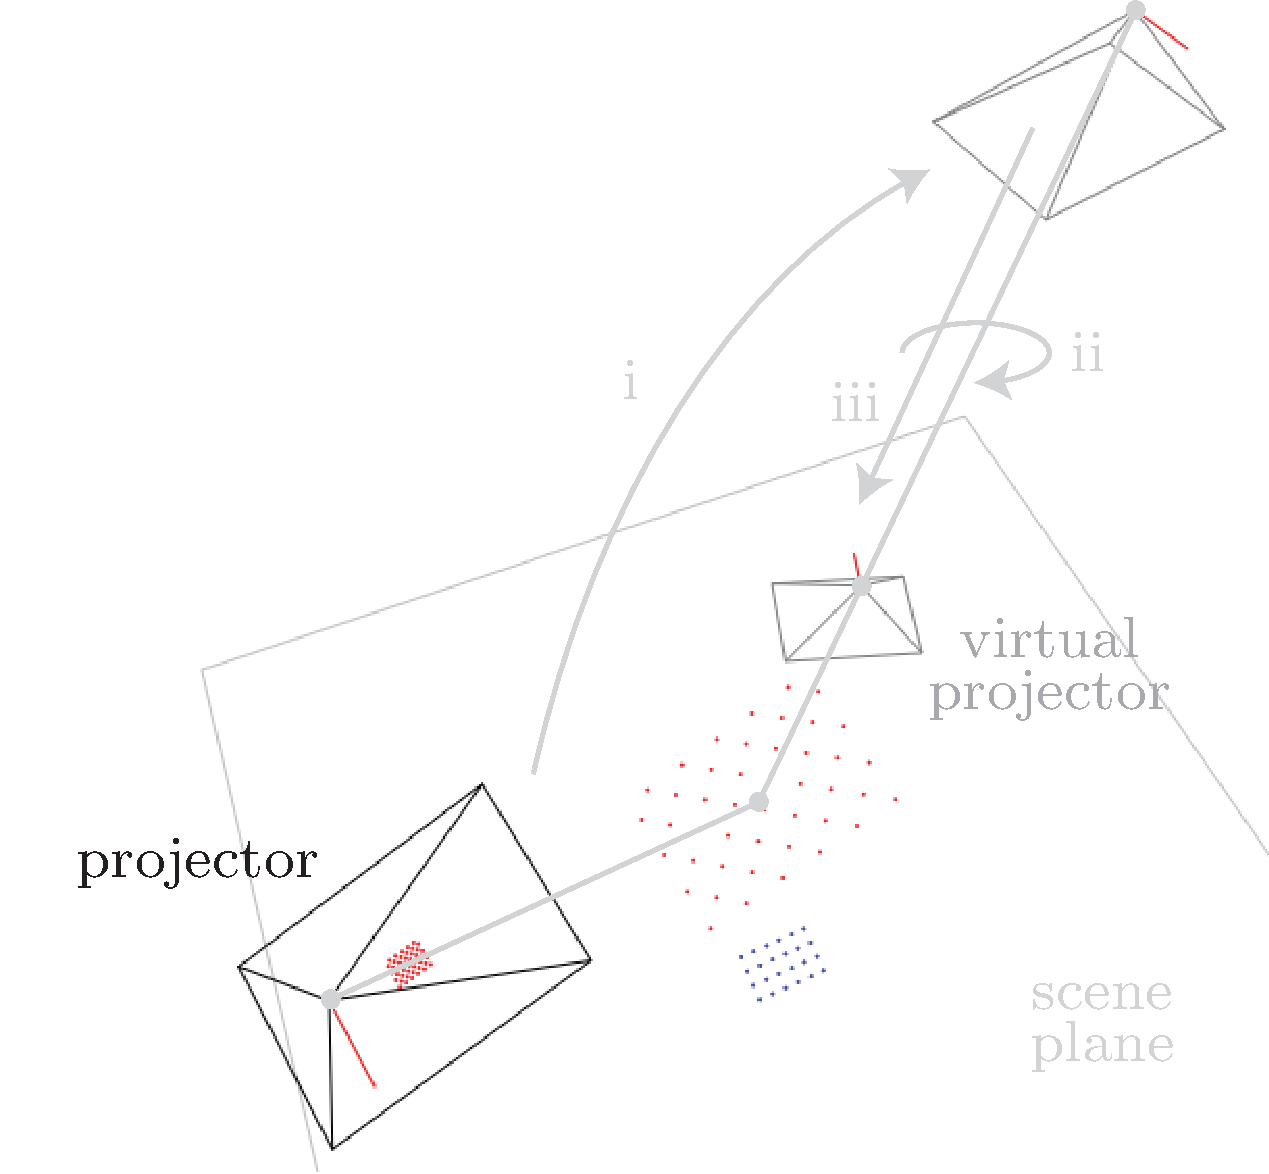
\includegraphics[height=5.25cm]{images/3_proj_.pdf}}}
    \qquad
    \subfloat[\centering View directly downwards to scene~plane.]{{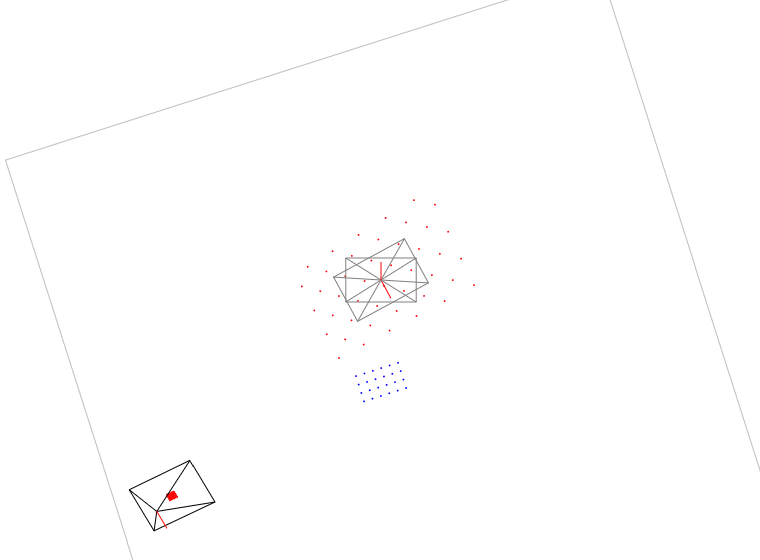
\includegraphics[height=5.25cm]{images/3_above3_proj.png}}}
    \caption{Obtaining the virtual projector. For a given target location, the virtual projector is obtained by (i) rotating the recovered projector (bottom left, frustum in black) about the point of intersection of its optical axis with the scene plane such that the optical axis be made parallel with the scene plane's normal vector, (ii) rotating the $X$- and $Y$-axes to align them with those of the virtual camera guaranteed---in contrast to the `downwards-facing' camera---to face \textit{directly} downwards to the scene plane (cf.\ Figure \ref{fig:virtualcam}), and (iii) translating along the normal direction to achieve the desired metric projected image dimensions. Note in (b) that the virtual projector's principal axes are aigned with those of the virtual camera in Figure~\ref{fig:virtualcam}(b).} %The virtual projector is thus rendered fronto-parallel with the ground plane and axially aligned with the virtual camera.
    \label{fig:virtualproj}
\end{figure}

\paragraph{Virtual projector} The placement of the virtual projector---for a given a target location---determines from which pose the image to be projected is to \textit{appear} to have been projected, with the effect correcting for projective distortions, placing the axes of the augmentation in accordance with the axes of the `downwards-facing' camera, and setting the dimensions of the augmentation in line with the desired target dimensions.  We carry out this placement according to a small handful of steps. It is in accordance with the $X$- and $Y$-axes of the `downwards-facing' camera that we wish to place the $X$- and $Y$-axes of the augmentation, since we wish to intuitively be able to use the rotation of the camera relative to the scene plane to set those axes. It is, however, only if the virtual projector be placed to face the scene plane directly that the projection will appear free of distortions; this is noteworthy, since a physical camera placed to face downwards is almost certain to not face downwards to the scene plane precisely. Accordingly, we rotate the recovered camera about its center of projection to align its optical axis\footnote{Strictly speaking, the optical axis is the back-projection of the principal point; in our usage, we understand it to refer to the ray through center of the image plane.} with the normal vector of the scene plane by applying the minimum arc-length rotation that relates the two, giving a \textit{virtual} camera facing directly downwards to the scene plane (cf.\ Figure~\ref{fig:virtualcam}). To obtain the virtual projector, we then (i) intersect the scene plane with the optical axis of the projector and rotate the projector's placement about that point of intersection, aligning the optical axis with the scene plane's normal vector, and (ii) align the $X$- and $Y$-axes with those of the virtual camera. Finally, we (iii) translate along the scene plane's normal, in order to satisfy the desired metric projected image dimensions; the height $h$ [m] above the ground plane at which the virtual projector is to be placed if the image---with original image width of $w_\text{im}$ [px]---is to be projected to the scene plane with a metric width of $w$ [m] is given by
\begin{equation}
h = w \times f_\text{proj} / w_\text{im},
\end{equation}
where $f_\text{proj}$ [px] is the focal length of the projector. These three steps are illustrated in Figure~\ref{fig:virtualproj}. The resulting virtual projector is thus rendered fronto-parallel with the scene plane---enabling projection to the scene plane absent of projective distortions---and projects to the scene plane in the desired scale and with the the $X$- and $Y$-axes of the augmentation set in accordance with those of the `downwards-facing' camera. %\footnote{A physical camera placed to face downwards is almost certain to not face downwards precisely; in contrast, we align the virtual camera's optical axis exactly with the scene plane's normal vector, rendering it genuinely fronto-parallel with respect to the scene plane.}

It is thus in the sense that we set the $X$- and $Y$-axes of the virtual projector to the $X$- and $Y$-axes of the virtual camera that we place the horizontal and vertical axes of the desired augmentations `in accordance' with the horizontal and vertical image axes of the `downwards-facing' camera; the placement of the camera thereby intuitively determines the principal axes according to which augmentations are to be placed. Note further that a consequence of placing the virtual projector by rotating about the point of intersection of the projector's optical axis with the scene plane is that \textit{the center of the projector's image plane remains invariant} to the placement of the virtual projector. A steerable mirror can be aimed with respect to a point projected from the center of the projector's image plane, thereby further facilitating placement.

\begin{figure}
    \centering
    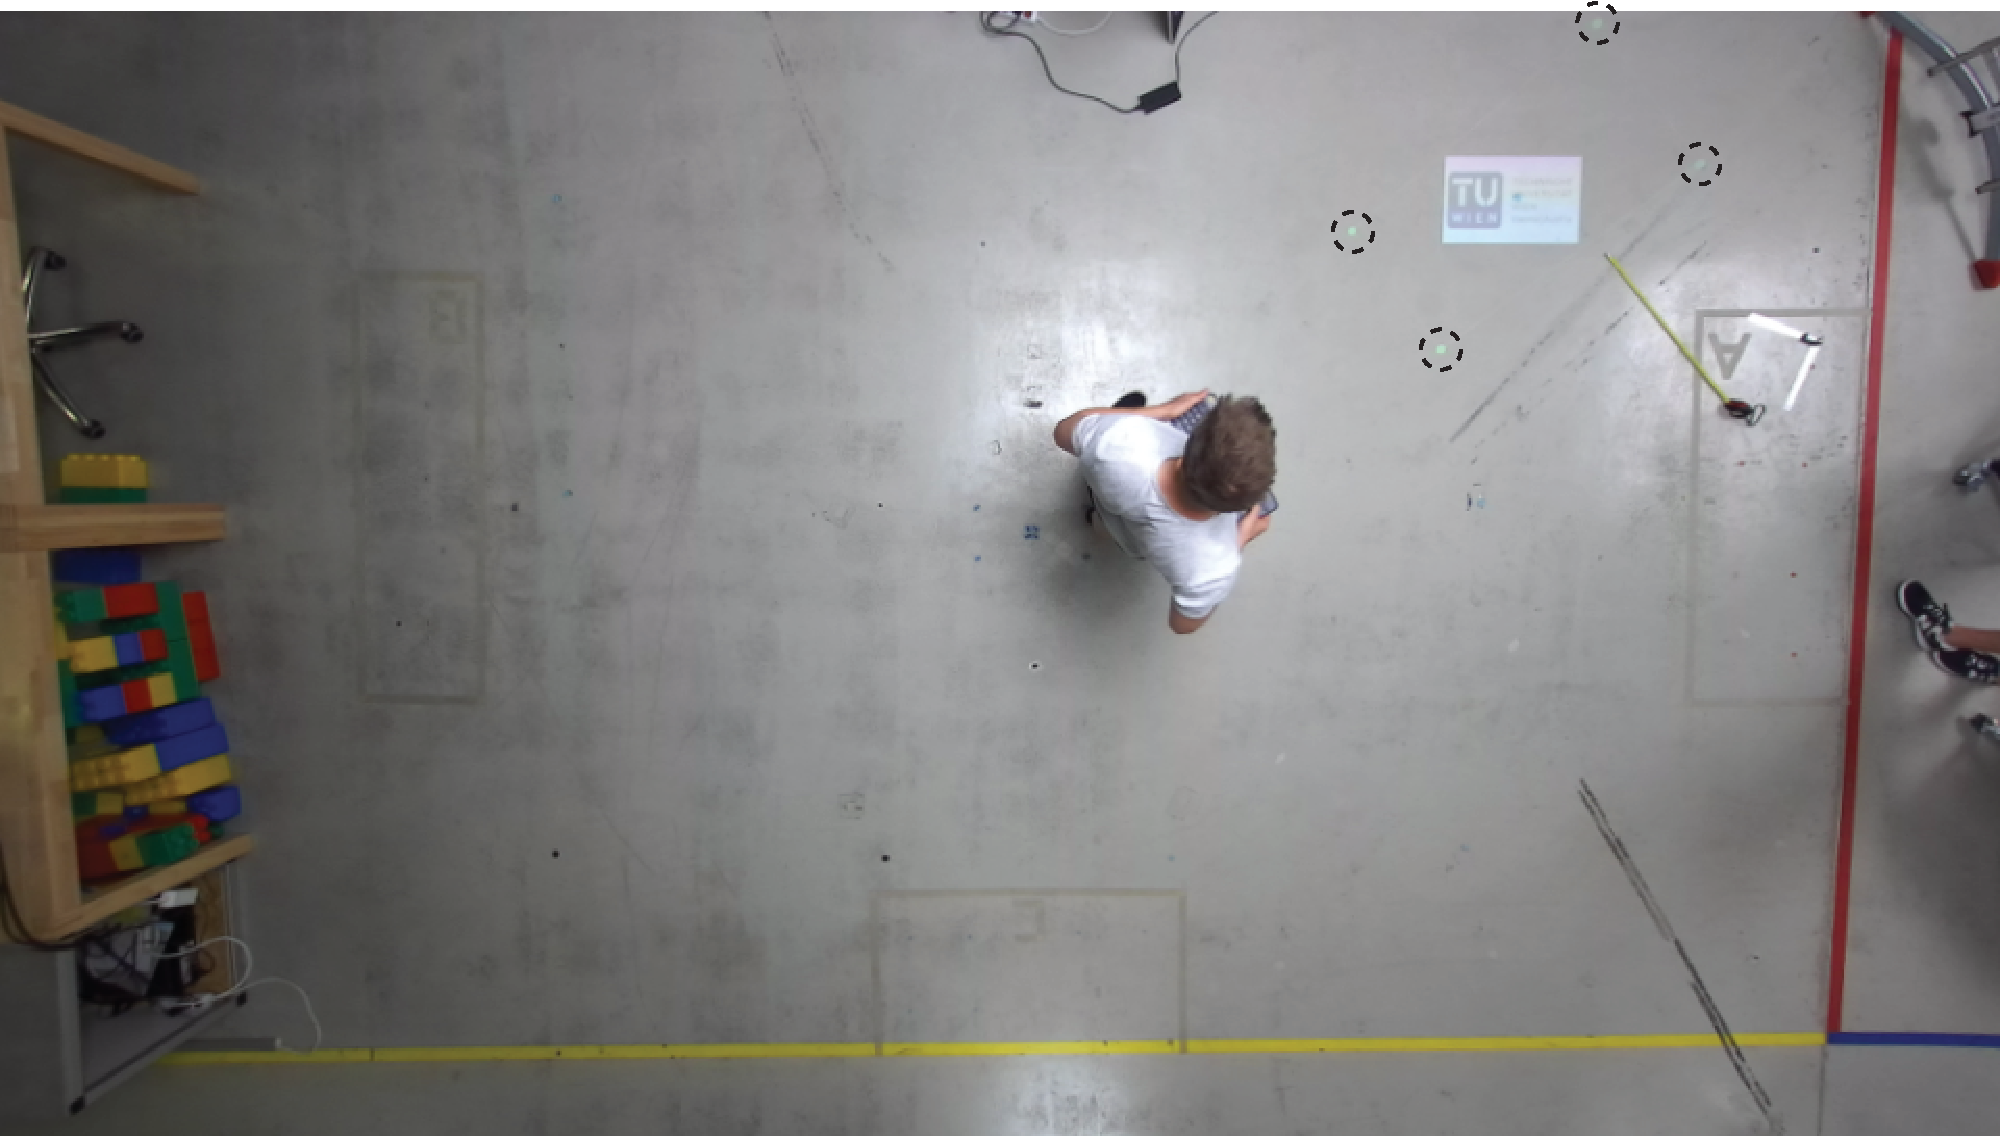
\includegraphics[height=4.5cm]{images/hans_undist_.pdf}
    \caption{Projection of the warped image from Figure \ref{fig:warp}(a) to corresponding target location at the upper-right corner of the floorspace, acquired by the `downwards-facing' camera. Note that besides correcting for projective distortions, the warp places the axes of the augmentation in accordance with the axes of the `downwards-facing' camera, and that the dimensions of the augmentation are in line with the desired target dimensions (50~cm~$\times$~31.25~cm). To provide context, the corners of the full projected image extent are projected to the floor in light green (emphasized with overlain dashed circles).}
    \label{fig:final_proj}
\end{figure}

\paragraph{Plane-induced homography} Let $\mathtt{K}_\text{proj}$ express the calibration matrix of the recovered projector and $(\mathtt{R}, \mathbf{t})$ the rigid body transformation that transforms points from the coordinate frame of the recovered projector to that of the virtual projector, for a given target location. Moreover, let $(\mathbf{n}^\top, -d)^\top \in \mathbb{P}^3$ give the scene plane, expressed in the coordinate frame of the recovered projector, where $\mathbf{n} \in \mathbb{R}^3$ is the scene plane's normal vector and $d = \mathbf{n}^\top\mathbf{X}$ for any point~$\mathbf{X} \in \mathbb{R}^3$ in the plane, so that $(\mathbf{n}^\top, -d) (\mathbf{X}^\top, 1)^\top = 0$. The transformation that warps the image to be projected---by the recovered projector to the scene plane---such that it appear as if were projected to the scene plane by the virtual projector (cf.\ Figures~\ref{fig:warp} and \ref{fig:final_proj}) is given the by the $3~\times~3$ matrix
\begin{equation}
\mathtt{H} = \mathtt{K}_\text{proj}\left(\mathtt{R} - \frac{\mathbf{t}\mathbf{n}^\top}{d}\right)\mathtt{K}_\text{proj}^{-1},
\label{homgen}
\end{equation}
a form of `plane-induced' 2D homography \cite{Hartley2004}. For convenience, we enable optional rotation of the image to be projected \textit{before} applying $\mathtt{H}$, about the image center; that rotation, parameterized in degrees, is thus in effect carried out---again intuitively---with respect to the ground plane.

\begin{figure}
    \centering
    \subfloat[\centering Hardware setup consisting of projector, steerable mirror system, `downwards-facing' camera (i.e., camera placed to face downards towards the scene plane, here the left view of a stereo camera).]{{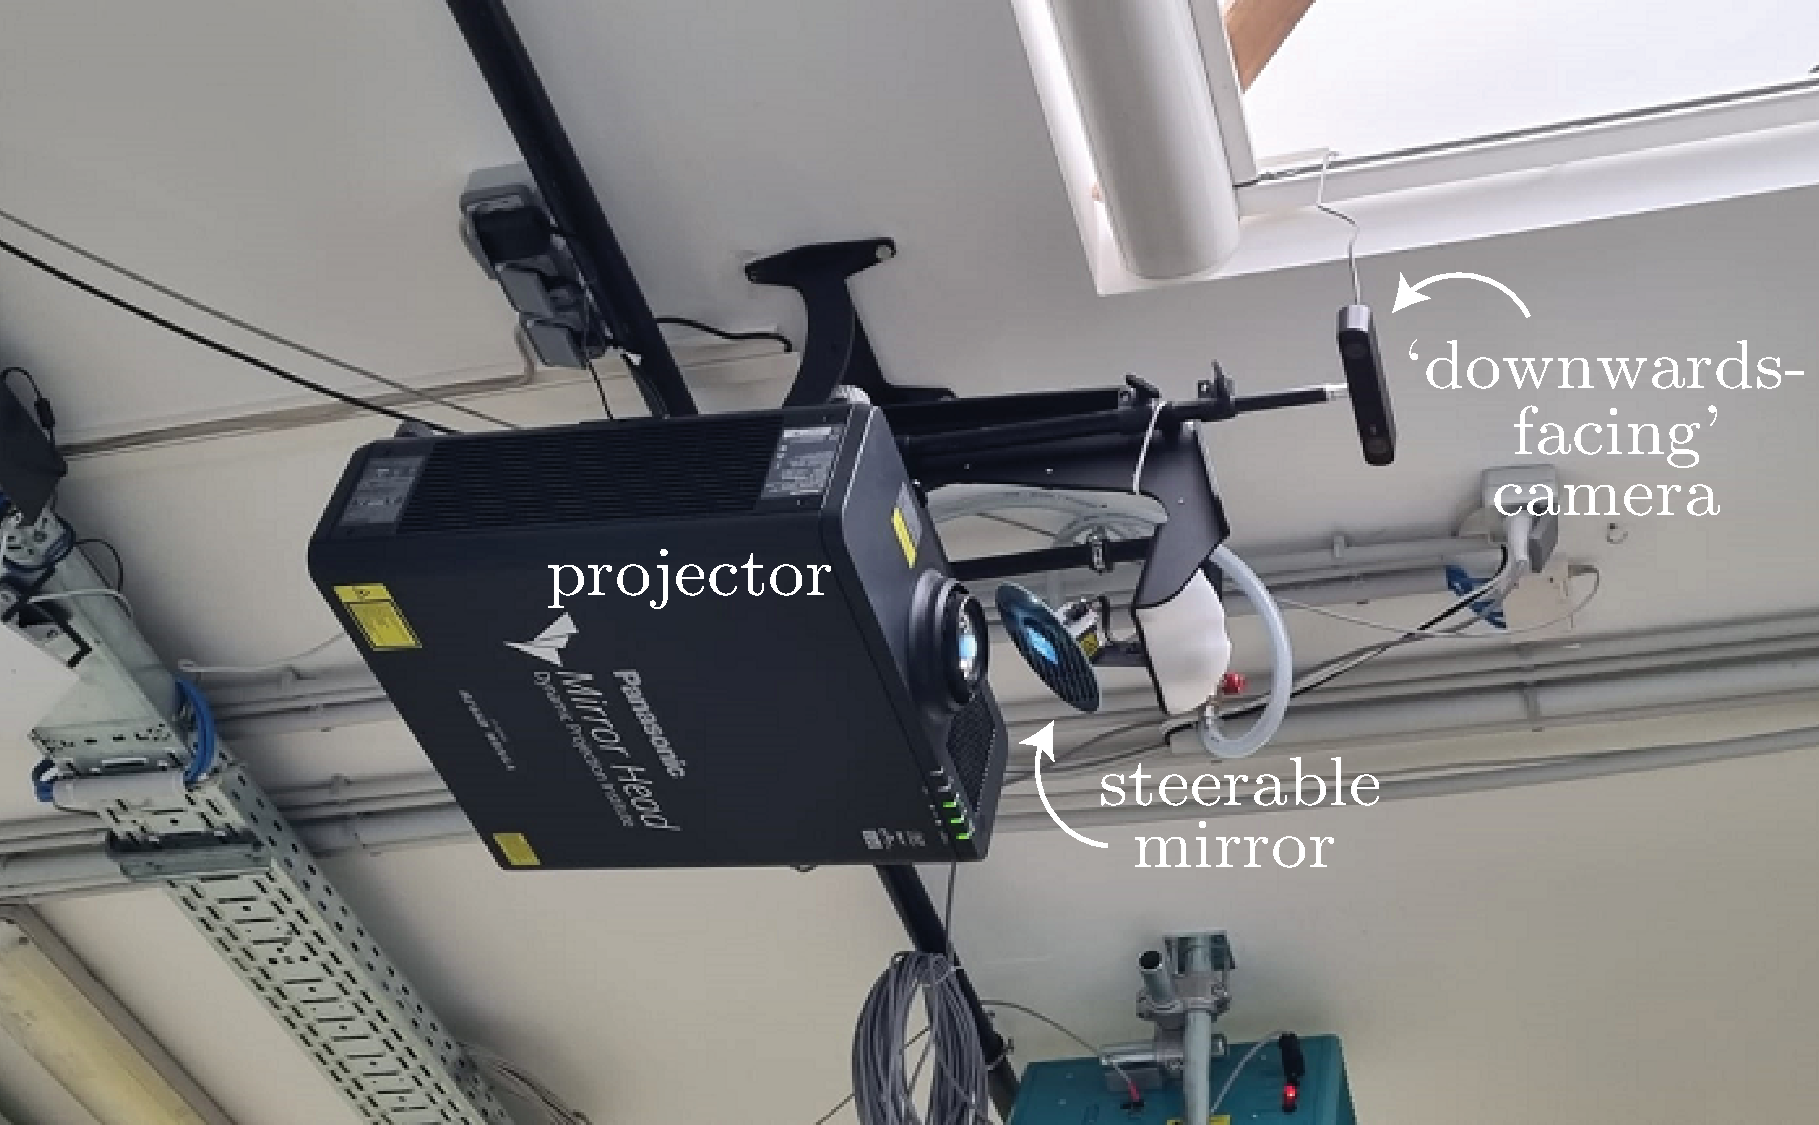
\includegraphics[height=5cm]{images/system3_.pdf}}}  %3.6
    \quad
    \subfloat[\centering Measurement for augmentation, using a steel rule and a digital angle gauge (enlargements on the right).]{{\includegraphics[height=5cm]{images/meas2_.pdf}}}
    \caption{Evaluation scenario. (a) Our hardware setup, comprised of a projector, a steerable mirror system, and a stereo camera, of which we used only the left view. (b) Example augmentation produced by projecting---to one of the 15 target locations across the floorspace considered in our evaluation, to the upper-left corner of our floorspace---an image warped using our approach. The digital angle gauge reads $89.6^\circ{}$ for the top-left corner, and the steel rule 49.9 cm for the bottom edge. Corners of the full projected image extent projected to the floor in light green to provide context. Note that blur has a minimal impact on the quality of the augmentation, and hence on the accuracy of the measurements.}
    \label{fig:eval}
\end{figure}

\section{Evaluation}

We evaluate our approach by using a 960 pixel~$\times$~600 pixel image of the TU Wien logo (cf.\ Figure \ref{fig:proj}(a)) to augment 15 locations across the floorspace at the Pilotfabrik\footnote{\url{https://www.pilotfabrik.at/}} of TU Wien, a collaborative space for research on Industry 4.0 topics situated in Vienna, Austria. We contrast our approach with a baseline approach involving manual keystone correction, by aiming with both approaches to place the same image of the TU Wien logo for each of the 15 locations, aligned with the principal axes of the floorspace (i.e., the yellow and red lines in Figure~\ref{fig:2d}(b)), absent of projective distortions, and with the same metric dimensions of 50~cm~$\times$~31.25~cm\footnote{The dimensions in pixels of the image we project are 960~$\times$~600; we chose for our experiments to set the projected metric length of the horizontal axis of the image to 50~cm, which implies 31.25~cm for the vertical axis if aspect ratio is to be preserved.}. All experiments were carried out by the same technician, experienced in both approaches.

The hardware setup employed in the evaluation (cf.\ Figure \ref{fig:eval}(a)) comprised a Panasonic PT-RZ660BE projector (Panasonic Corporation, Japan) with a steerable mirror system---used in our experiments to point the projection to each of the 15 locations---manufactured by Dynamic Projection Institute (Dynamic Projection Institute, Austria) \cite{rupprecht2020information,Rupprecht2021}. The steerable mirror system was bundled with the MDC-X software for steering the mirror, loading imagery, and optionally carrying out manual keystone correction, such that each position and (warped) image can be registered as a preset. In addition, we used a Stereolabs Zed 2 stereo camera (Stereolabs Inc., France) as our `downwards-facing' camera, making use of only its left view. The floorspace used for our experiments measured dimensions of ca.\ 6~m~$\times$~4~m; the projector and camera were mounted at approximately the center of this space, at a height of ca.\ 3.5 m. At this height, the pixel size (i.e., length or width of a pixel if projected to the scene plane) of the camera was ca.\ 3.5 mm.

\begin{table}[ht!]
\caption{Mean absolute error (MAE) and maximum absolute error in units of centimeters, with respect to the four sides (top, bottom, left, right) of the 15~augmentations produced using our approach for 15 target locations spread across the floorspace, respectively. Errors were computed against intended augmentation dimensions of 50~cm~$\times$~31.25~cm (i.e., 50~cm for top and bottom, 31.25~cm---rounded to 31.3~cm for the purposes of the computing the errors---for left and right).} %Note that absolute errors in no instance exceeded 1~cm for any side of any of the 15~augmentations.
\label{table:length}
\centering
{\small
\begin{tabularx}{7.4cm}{r p{1cm} p{1cm} p{1cm} p{1cm}}
\toprule
  & Top & Bottom & Left & Right \\
\midrule
MAE {\tiny[cm]} & 0.23 & 0.17 & 0.22 & 0.2 \\
%Min AE {\tiny[cm]} & 0.0 & 0.0 & 0.0 & 0.0 \\
Max AE {\tiny[cm]} & 0.8 & 0.6 & 0.5 & 0.5 \\
\bottomrule
\end{tabularx}}
\end{table}

\paragraph{Manual approach} Having pointed the steerable mirror to the desired location, manual keystone correction using the MDC-X software involves warping the image to be projected by manipulating the corners of the image until the desired effect is produced on the projection surface. In order to provide a template for manually carrying out keystone correction, we prepared a rectangular 50~cm~$\times$~31.25~cm cutout of cardboard. For each target location, we placed this piece of cardboard in a manner that its axes were aligned with the principal axes of the floorspace; we then manually warped the image of the TU Wien logo for the given target location so that any corner of the augmentation deviated by at most 1 cm from the corresponding corner of the template. End-to-end, the process of setting the presets in the MDC-X software having carried out keystone correction manually took ca.\ 32 min for the 15 target locations.

\begin{table}[ht!]
\caption{Mean absolute error (MAE) and maximum absolute error in units of degrees, with respect to the top-left and bottom-right corners of the 15~augmentations produced using our approach for 15 target locations spread across the floorspace, respectively. Errors computed in terms of deviation from $90^\circ{}$.}
\label{table:angle}
\centering
{\small
\begin{tabularx}{6.75cm}{r p{1.95cm} p{1.95cm}}
\toprule
  & Top Left & Bottom Right \\
\midrule
MAE {\tiny[deg]} & 0.17 & 0.32 \\
%Min AE {\tiny[deg]} & 0.0 & 0.0 \\
Max AE {\tiny[deg]} & 0.9 & 0.5 \\
\bottomrule
\end{tabularx}}
\end{table}

\paragraph{Our approach} We began by carrying out a calibration of the camera, acquiring 10~camera calibration images (cf.\ Section~\ref{sec:approach:geometry}) of a chessboard calibration pattern with $6~\times~4$ corners ($7~\times~5$ squares) and feeding the images as input to our camera calibration module. Separately, for each of the 15~target locations, we produced a projector calibration image (cf.\ again Section~\ref{sec:approach:geometry}) by projecting a $11~\times~4$ asymmetrical circle pattern image to the target location in question by directing the projection using the steerable mirror, placing a chessboard pattern beside the projected pattern, and acquiring the image using the `downwards-facing' camera. We then fed these images alongside the output of the camera calibration module to our projector calibration module. For each of the target locations, the target location was registered in the MDC-X software as a preset. The output of the projector calibration module is a homography per input projector calibration image (cf.\ Section~\ref{sec:approach:homography}). Next, we warped the image of the TU Wien logo to the respective target locations using the corresponding homography, using a third dedicated custom module responsible for warping an image according to a homography. These warped images were finally imported into the MDC-X software and associated with their respective target location presets (cf.\ Figure~\ref{fig:eval}(b)).

Tables~\ref{table:length} and \ref{table:angle} give the errors in measured lengths and angles, respectively, with respect to the intended quantities. Lengths were measured using a steel rule for the top, bottom, left, and right sides of the 15~augmentations; angles were measured using a digital angle gauge at the 15~augmentations' top-left and bottom-right corners. Note that absolute errors in lengths in no instance exceeded 1~cm for any side of any of the 15~augmentations, or $1^\circ{}$ for any of the measured corners. The total amount of time expended for carrying out all the above steps amounted to ca.\ 20~min, with ca.\ 2 min going to acquisition of the camera calibration images, and ca.\ 5 min going to that of projector calibration images. The remainder of the time was spent running our modules or working with the MDC-X software. Note that once the camera is calibrated, that calibration can be reused if the camera's optics remain fixed, notably if no change is made to the zoom factor or focus settings of the camera.

\section{Conclusion}

We presented a spatial AR system for planar scenes that produces the effect of keystone correction analytically as a function of the geometry relating projector and scene plane, exploiting a steerable mirror system to enable augmentation exceeding the bounds of the projector's own immediate field of view. Our method produces this effect in a manner that enables intuitive placement of the augmentations in accordance with the $X$- and $Y$-axes of a camera placed to face downwards towards the scene plane. Moreover, our method allows for specifying the desired dimensions of augmentations in metric terms, thus enabling consistent scaling. Our evaluation demonstrated our approach to produce compelling results---with mean and standard deviation of errors in measured lengths within the `downwards-facing' camera's pixel size---at less time than a more cumbersome manual approach to keystone correction.

A natural extension of this work would be to consider the impact of varying calibration patterns, their dimensions, and their scale relative to the camera, or to consider the impact of the `downwards-facing' camera's pixel size. Still another would be to address the augmentation of non-planar scenes. To handle non-planar scenes would call for a change in how scene geometry is recovered and how warping of the image to be projected is carried out; the methodology we proposed for projector calibration could, however, be left unchanged.

\section{Acknowledgments}

This work was supported by the Austrian Research Promotion Agency (FFG) through its endowed professorship in Human Centered Cyber Physical Production and Assembly Systems at TU Wien (FFG-852789).

\bibliography{mybibfile}

\end{document}

% idea for next work: LM-based approach to globally recover scene plane from projected patterns (try to make a patent of this!)... compute intersection of optical axes of all recovered projectors - it is about this point that the projector can be steered in terms of angles; once scene plane is availabe, intrinsics of projector are available, and the 'steering point' is available, we can have a GUI with which you click on an undistorted image of the scene plane to control the steerable mirror
